\section{Breve introducción a la mecánica estadística}

En la mayoría de los experimentos que se realizan en un laboratorio se obtiene 
una serie de mediciones sobre sistemas macroscópicos, usualmente constituidos por 
más de 10$^{20}$ moléculas, durante un período de tiempo a las cuales luego se 
les realiza un promedio. La mecánica estadística ofrece una interpretación de 
las propiedades del equilibrio de sistemas macroscópicos a partir de una teoría 
molecular aplicada a su configuración microscópica ~\cite{hill1986}.

Si se quisiera calcular alguna variable mecánica de un sistema termodinámico a
partir de consideraciones moleculares tendríamos que hacerlo durante un período
de tiempo largo para suavizar las fluctuaciones y para que fuera independiente
del paso inicial a la hora de realizar el promedio. Dado el gran número de 
moléculas interactuantes entre sí en estos sistemas, este cálculo está fuera de
alcance tanto en una consideración cuántica como en una clásica. Una alternativa
para solucionar esto es conectar el promedio temporal de la variable mecánica de
interés con el promedio de ensambles, donde un ensamble es simplemente una 
colección de un número muy largo de sistemas construidos de manera tal que 
reproducen las propiedades termodinámicas del sistema en cuestión. Si bien todos
los sistemas en el ensamble son idénticos desde el punto de vista termodinámico,
no lo son en sus configuraciones moleculares. De esta manera ahora se tiene
que el valor promedio de la variable mecánica en estudio se realiza sobre estas 
replicas del sistema en vez de sobre su evolución temporal.

\subsection{Ensambles}

Algunos de los ensambles termodinámicos más relevantes son:
\begin{enumerate}
    \item \textit{Ensamble microcanónico (NVE)}, un sistema aislado en el cual el 
        número de partículas, el volumen y la energía permanecen constantes.
    \item \textit{Ensamble canónico (NVT)}, un sistema cerrado, con una cantidad
        fija de partículas y volumen constante, en contacto con un baño de 
        temperatura lo suficientemente grande de manera tal que la misma permanece 
        constante.
    \item \textit{Ensamble gran canónico ($\mu$VT)}, un sistema abierto en el que
        el volumen está fijo, se está en contacto con un baño de temperatura y
        además se permite el intercambio de partículas con un reservorio.
    \item \textit{Ensamble isotérmico-isobárico (NPT)}, en este sistema el número
        de partículas está fijo y en contacto con un baño de temperatura y un
        pistón que permite variar el volumen para mantener la presión constante.
\end{enumerate}

\subsection{Hipótesis ergódica}

El primer postulado de la Mecánica estadística presentado en esta tesis es 
referido como la \textbf{hipótesis ergódica} y nos dice que \textit{El promedio 
temporal de una variable mecánica $M$ en el sistema termodinámico de interés es 
igual al promedio de ensambles de M, en el límite del conjunto de ensambles que 
tiende a infinito, siempre que los sistemas del conjunto de ensambles reproduzcan 
el estado termodinámico y el entorno del sistema real de interés}. Es decir que
es lo mismo calcular el promedio en la evolución temporal que en una cantidad 
grande estructuras instantáneas representativas del sistema. Para poder aplicar
este postulado se necesita conocer la probabilidad relativa de cada uno de los 
estados presentes en el ensamble.

\subsection{Postulado de igual probabilidad a priori}

El segundo postulado de la Mecánica estadística presentado se refiere a esto
último y establece que \textit{En un conjunto de ensambles representativo de un 
sistema termodinámico aislado, los sistemas del conjunto de ensambles se distribuyen 
uniformemente, es decir, con igual probabilidad o frecuencia, sobre los posibles 
estados con los valores especificados de dicho sistema termodinámico aislado}.
En otras palabras, cada estado esta representado por la misma cantidad de sistemas
en el ensamble.


\section{Dinámica molecular}\label{md}

La dinámica molecular (MD, de sus siglas en inglés, \textit{molecular dynamics})
es una técnica de simulación computacional que considera un sistema de $N$
partículas atómicas, que interactúan a través de un campo de fuerzas newtoniano,
de las cuales se obtiene su evolución temporal. La misma permite obtener
propiedades termodinámicas macroscópicas de un sistema en equilibro a partir de 
cantidades microscópicas ~\cite{frenkel2001, allen2017}.

Para entender mejor como trabaja esta técnica de simulación es conveniente ver
cómo funciona su código fuente, un diagrama de flujo del mismo es presentado en 
la figura \ref{fig:esquema_md}, donde cada una de sus partes se amplía en la 
siguiente enumeración:
\begin{enumerate}
    \item \textbf{Inicialización del sistema}: se especifican las posiciones y
        velocidades iniciales de los átomos. También se elije un paso temporal, 
        un radio de corte para las interacciones y las condiciones de contorno que
        se van a respetar a lo largo de la simulación. 
    \item \textbf{Cálculo de fuerzas}: con las posiciones especificadas se
        calcula la fuerza sobre cada uno de los átomos a través del campo de 
        fuerzas elegido.
    \item \textbf{Integración de las ecuaciones de movimiento}: se integran las
        ecuaciones de Newton mediante algún integrador que obtiene las posiciones
        y velocidades del paso temporal siguiente a partir del actual.
    \item \textbf{Cómputo de propiedades termodinámicas}: se realizan los
        cálculos de distintas cantidades de interés, como las energías potencial
        y cinética, la presión y la temperatura.
    \item De ser necesario, se aplica algún \textbf{termostato o barostato}
        para realizar simulaciones en el ensamble termodinámico deseado.
    \item \textbf{Evolución temporal}: se incrementa el tiempo adhiriendo un
        paso temporal y se vuelve al cálculo de las fuerzas con las nuevas 
        configuraciones.
\end{enumerate}

\begin{figure}
    \centering
    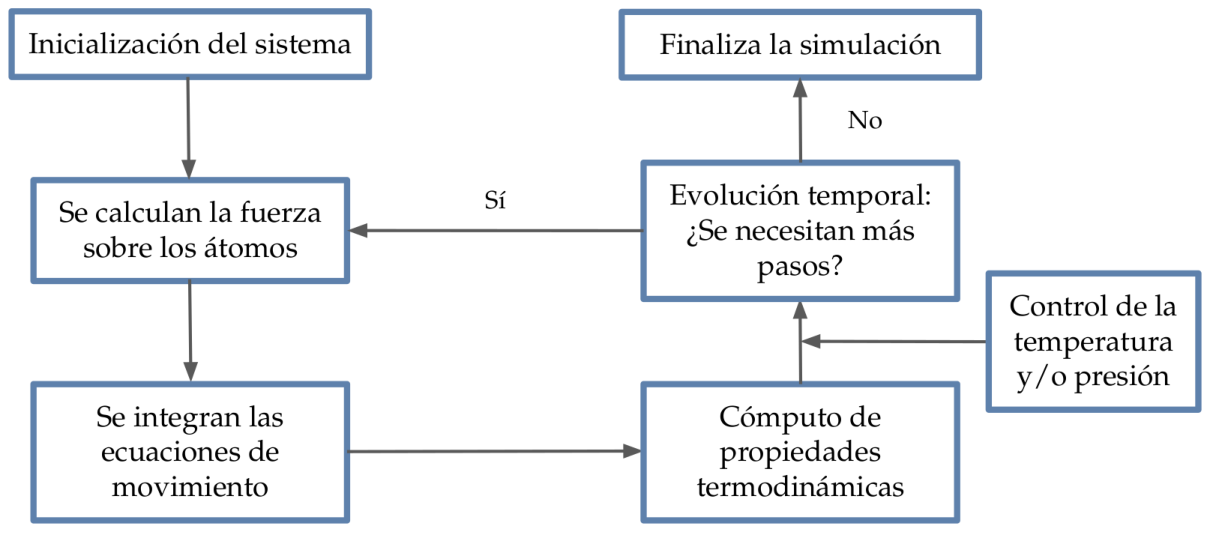
\includegraphics[width=\textwidth]{metodos/esquema_de_dinamica_molecular.pdf}
    \caption{Esquema de un diagrama de flujo de una dinámica molecular usual.}
    \label{fig:esquema_md}
\end{figure}

A continuación se especifican cada una de dichas partes con mayor detenimiento.

\subsection{Configuraciones iniciales}

Si bien las posiciones iniciales de algunos sistemas pueden reproducirse a partir
de los vectores de red de estructuras cristalinas (\textit{simple cubic}, 
\textit{body-centered cubic}, \textit{face-centered cubic}), otros casos de
interés, en los cuales hay más de un elemento involucrado, involucran celdas 
unidad más complicadas que han sido calculadas y optimizadas mediente la Teoría
del funcional de la densidad (DFT, de sus siglas en inglés, density functional
theory). Realizar estos cálculos suele ser una tarea computacionalmente costosa 
y que requiere intervención de científicos especializados, para evitar esto
existe una base de datos ampliamente utilizada en el ámbito académico y en
la industria, Materials Project \cite{materials_project}, que recopila los datos
que existen sobre estas estructuras cristalinas, realiza nuevos cálculos y está 
abierta a la comunidad para su uso y colaboración. Antes de que los datos se
cargen en la página, los mismos son comparados con resultados experimentales 
para determinar si están dentro de un rango de validez definido. En esta tesis
en particular, fueron utilizadas distintas estructuras cristalinas de esta base de
datos como condiciones iniciales para las posiciones y el tamaño de la celda de 
simulación.

Las velocidades de los átomos suelen ser generadas de manera aleatoria, a través
de un generador de números pseudo-aleatorio, tomando como argumento una semilla 
para la reproducibilidad de la simulación y una temperatura deseada para el
sistema. Estos números suelen ser generados de una distribución gaussiana, donde
el centro se lo fija a cero para que no haya una velocidad en el centro de masa
y el ancho está relacionado a la temperatura.

\subsection{Condiciones de contorno}

Además de dar la configuración inicial de los átomos, es necesario especificar si
los mismos se encuentran dentro de una celda de simulación con un largo tamaño en
particular para cada una de las direcciones del sistema o si no interactúan fuera
del borde de la estructura que conforman los mismos. En el primero de los casos
se tienen condiciones periódicas de contorno (PBC, \textit{periodic boundary 
conditions}), lo que se busca con ellas es reproducir un sistema infinito, para
que no existan efectos de borde, y consiste en considerar que los átomos se 
encuentran dentro de una celda unidad de una red infinita de celdas idénticas; en
donde si un átomo sale por un extremo de la celda, ingresa por el opuesto. Una
condición que debe cumplir esta celda es que su tamaño en cada una de las 
direcciones debe ser mayor al radio de corte de las interacciones entre los átomos. 
Por otro lado, el segundo de los casos es útil considerarlo cuando se 
tienen nanoestructuras en las cuales los átomos están ordenados de cierta forma 
que globalmente representan una forma definida y no pueden ser consideradas como
una red infinita.

\subsection{Potenciales interatómicos}

Existen una gran variedad de potenciales interatómicos para utilizar en dinámicas
moleculares. La elección de cada uno de ellos depende del sistema de estudio ya
que algunos potenciales representan de mejor manera gases y otros metales. A pesar
de esto, un potencial interatómico suele tener contribuciones atractivas y
repulsivas, según la distancia, con un mínimo que se encuentra a la distancia del
enlace entre dos átomos. Como ejemplo se toma un potencial interatómico de 
Lennard-Jones (12-6), dado por la siguiente expresión
$$
V_{LJ} = 4\varepsilon \left[ \left( \frac{\sigma}{r} \right)^{12} - 
                             \left( \frac{\sigma}{r} \right)^{6} \right],
$$
donde $r$ es la distancia entre dos átomos, $\varepsilon$ indica la profundidad 
del pozo del potencial que se encuentra en $r_m = 2^{1/6} \sigma$, $\sigma$ es el
radio del átomo. En la figura \ref{fig:lj} 
\begin{figure}
    \centering
    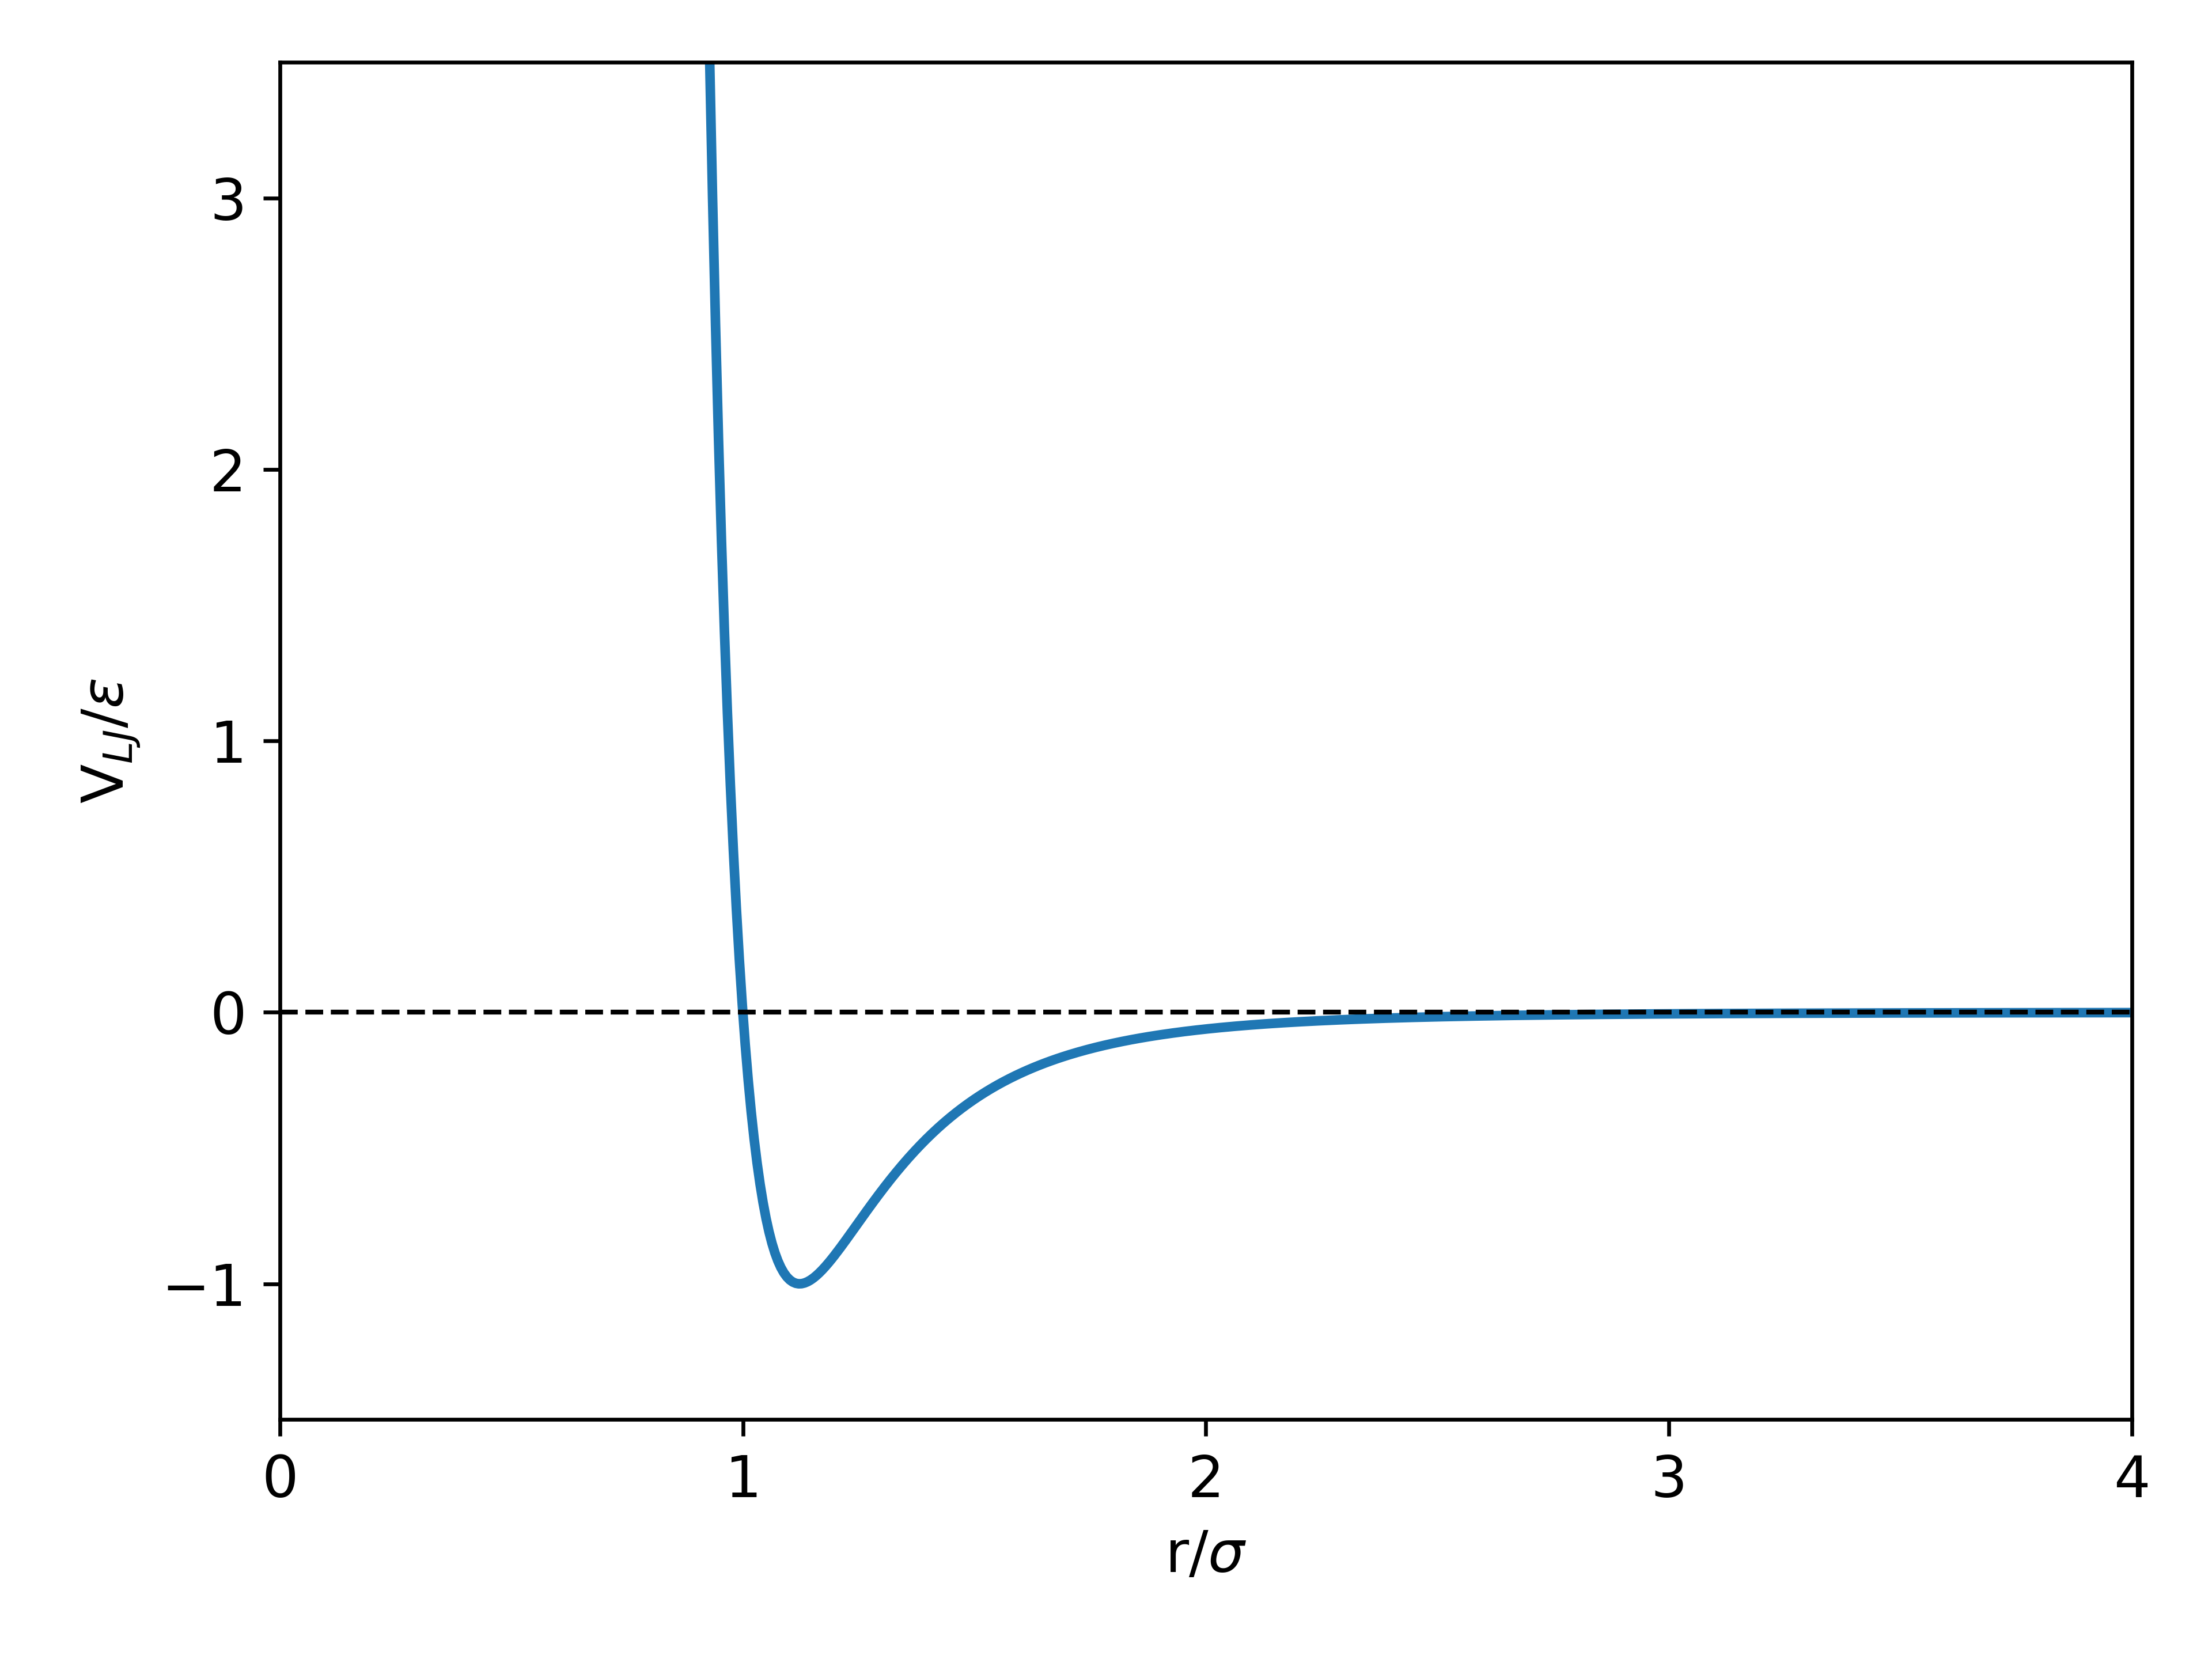
\includegraphics[width=0.7\textwidth]{metodos/lj.png}
    \caption{Gráfico de un potencial de Lennard-Jones.}
    \label{fig:lj}
\end{figure}
se muestra el comportamiento de este potencial, si la distancia entre dos
átomos es menor a $r_m$ entonces se repelen, si es mayor a dicha distancia, se 
atraen. Cuando la distancia entre dos átomos es infinita, los mismos no 
interactúan, en el caso práctico se define una distancia de corte, conocida como
el \textit{radio de corte}, $r_{cut}$, a partir de la cual se considera que el 
potencial es nulo. Para evitar discontinuidades en este punto se suelen utilizar 
distintas técnicas como el truncado y desplazado o se multiplica al potencial 
al rededor de dicho punto por una función \textit{smooth}, que hace que el 
potencial se iguale suavemente a cero.

Una vez que el potencial interatómico está bien definido, para calcular la fuerza
que actúa sobre el átomo $i$ es necesario computar la fuerza de a pares con todos
los átomos $j$ del sistema. Para esto es necesario calcular las distancias,
considerando la imagen mínima si las condiciones de contorno son PBC, y ver si
las mismas son mayores o menores a $r_{cut}$, si la distancia es mayor entonces
la contribución de esa interacción es igual a cero y si es menor se computa la 
fuerza a través del potencial de la siguiente manera
$$
f_x(r) = - \frac{\partial V(r)}{\partial x}
       = - \left( \frac{x}{r_{ij}} \right) \cdot \left( \frac{
                                       \partial V(r)}{\partial r} \right)
$$
donde $r$ es la distancia entre los átomos, $x$ la componente en alguna de
las direcciones definidas para el sistema.

A continuación se presentan dos potenciales interatómicos del estado del arte que
fueron utilizados a lo largo de esta tesis.

\subsubsection{ReaxFF}

\subsubsection{DFTB}

\subsection{Integrador}

La funcionalidad que cumple un integrador en un código de dinámica molecular es
la de evolucionar las velocidades y las posiciones de los átomos una vez que 
ya se conocen las fuerzas que se aplican sobre cada una de ellas. Un integrador
estándar, utilizado en esta tesis, fue el \textit{velocity Verlet}. El mismo 
conserva la energía total del sistema si no está siendo aplicado ningún termostato
o barostato que altere el ensamble. Para las posiciones se tiene una
actualización de las mismas, a partir del paso anterior, como un desarrollo de
Taylor
$$
r(t+dt) = r(t) + v(t) dt + \frac{f(t)}{2m} dt^2,
$$
donde $dt$ es el paso temporal y $m$ la masa en cuestión. Para las velocidades se
tiene
$$
v(t+dt) = v(t) + \frac{f(t+dt)+f(t)}{2m} dt,
$$
es importante notar que para calcular la velocidad del paso temporal siguiente se
necesita tener computadas las fuerzas anteriores y posteriores, por lo cual
primero se calculan las posiciones y, a partir de ellas, las fuerzas.

Una característica a destacar de este integrador, además de conservar la energía
total del sistema, es que soporta una elección de pasos temporales más grandes
que integradores anteriores, esto hace que se simule el mismo tiempo real con 
menos pasos y por lo tanto menos cómputo de fuerzas, que es la parte, 
computacionalmente hablando, más costosa del código.

\subsection{Cómputo de propiedades termodinámicas}

Una vez que ya se conocen las posiciones, velocidades y fuerzas de todos los 
átomos se tiene toda la información necesaria para computar distintas
cantidades de interés, el cómputo de cada una de ellas dependerá del ensamble en
el cual se están realizando las simulaciones.

Las energías que contribuyen a la energía total son dos, la potencial y la
cinética. La primera de ellas viene dada por por distintas contribuciones de
pares, ángulos, enlaces, etc, dependiendo de que tan complejo sea el campo de 
fuerzas utilizado. En el caso de que la interacción sea solo de a pares, la
energía potencial puede calcularse de la siguiente forma
$$
E_{pot} = \sum_{i < j} u(r_{ij}),
$$
donde $u(r_{ij})$ es la contribución proveniente de la interacción entre los 
átomos $i$ y $j$.

Por otro lado, la energía cinética traslacional puede calcularse a partir de las
velocidades de cada uno de los átomos como
$$
E_{cin} = \frac{1}{2} \sum_{i=1}^{N} m_i v_i^2, 
$$
donde $m_i$ es la masa del átomo $i$ y $v_i^2$ el módulo de su velocidad. 

También suele ser de interés obtener el valor de la temperatura y de la presión
del sistema. La temperatura en un paso de la simulación puede calcularse 
utilizando que
$$
k_B T = \sum_{i=1}^N \frac{m_i v_i^2}{N_f},
$$
donde $k_B$ es la constante del Boltzmann y $N_f$ los grados de libertad,
aproximados usualmente por $3N$ para sistemas lo suficientemente grandes. Por 
último, la presión puede calcularse como 
$$
P = \rho k_B T + \frac{1}{d V} \left\langle \sum_{i<j} \mathbf{f}(\mathbf{r}_{ij}) 
                                              \cdot \mathbf{r}_{ij} \right\rangle,
$$
donde $\rho$ es la densidad, $d$ la dimensión y $V$ el volumen del sistema. El
segundo término es conocido como el virial, donde $r_{ij}$ y $f(r_{ij})$ son las 
distancias y las fuerzas entre los átomos $i$ y $j$.

\subsection{Termostatos y barostatos}

Debido a que la dinámica molecular usual se realiza en el ensamble NVE y la 
mayoría de los experimentos con los cuales se pueden comparar resultados se 
realizan a temperatura y/o presión constante, es necesario introducir distintos
termostatos y barostatos que permitan controlar estos parámetros en las 
simulaciones realizadas. 

Desde el punto de vista de la mecánica estadística a un sistema se le puede 
imponer una temperatura si se lo pone en contacto con un baño térmico lo 
suficientemente grande. En dicho caso la probabilidad de encontrar al sistema en
un estado de energía viene dada por la distribución de Maxwell-Boltzmann,
\begin{equation}\label{eq:mb}
P(v) = \left( \frac{\beta}{2\pi m} \right)^{3/2} exp(-\beta v^2 / (2m)),
\end{equation}
donde $\beta$ es la energía térmica $k_BT$. Esto quiere decir que la velocidad de
un átomo no se mantiene constante cuando está en contacto con un baño térmico, si 
no que la misma puede fluctuar y la fluctuación va a depender de dicha temperatura
de la siguiente forma
$$
\sigma_T^2 = \frac{2}{3 N} \langle T \rangle_{NVT}^2,
$$
que proviene de calcular el segundo y el cuarto momento de la ecuación \ref{eq:mb}.

De manera análoga puede dejar de pensarse al volumen como constante y empezar a
pensar que el mismo es una variable cuando el sistema está acoplado a un pistón.

Distintos termostatos y barostatos fueron utilizados durante esta tesis, los mismos 
se introducen a continuación.

\subsubsection{Langevin}

Si se considera la ecuación de Langevin \cite{schneider1978}
\begin{equation}\label{eq:langevin}
    m_i \dot{v_i} = F_i - m_i \gamma v_i + R_i(t),
\end{equation}
donde $F_i$ es la fuerza con la que interactúan los átomos entre sí, $\gamma$ la
constante de fricción y $R_i(t)$ es una variable estocástica con media cero 
y que cumple
$$
\left\langle R_i(t) R_j(t+t') \right\rangle = 2m_i \gamma_i k_B T \delta(t') \delta_{ij}.
$$
Para aplicar este termostato, y simular a temperatura constante, en conjunto con 
el integrador \textit{velocity Verlet} se tienen que considerar tres parametros
\cite{kroger2005} a la hora de actualizar las velocidades y las posiciones como
$$
a = \frac{2 - \xi dt}{2 + \xi dt},
$$
$$
b= \sqrt{k_B T_0 \xi \frac{dt}{2}},
$$
$$
c= \frac{2 dt}{2 + \xi dt}
$$
donde $\xi$ es el factor de fricción, es decir, con qué intensidad interacciona 
el sistema con el baño térmico. Se tiene entonces una actualización se la siguiente
manera
$$
v(t+dt) = a v(t) + b \eta + \frac{f(t+dt)+f(t)}{2m} dt,
$$
$$
r(t+dt) = r(t) + c v(t) dt
$$
donde $\eta$ es una distribución gaussiana de números aleatorios con media 0 y
varianza 1. 

\subsubsection{Berendsen}

El termostato de Berendsen \cite{berendsen1984} puede derivarse si se considera 
la ecuación \ref{eq:langevin} sin el término estocástico y se hace una elección
en particular de la constante de fricción. Dicha ecuación de movimiento modificada
representa un escaleo de velocidades, 
$$
v(t) = \lambda v(t),
$$
por paso temporal, donde
$$
\lambda = \sqrt{1 + \frac{dt}{\tau_T} \left( \frac{T_0}{T} - 1 \right)}
$$
produce un cambio de temperatura igual a
$$
\frac{dT}{dt} = \frac{1}{\tau_T} (T_0 - T)
$$
donde $T_0$ es la temperatura de referencia y  $\tau_T$ es la constante de
acoplamiento con el baño térmico y tiene las mismas unidades que el paso temporal.

Para considerar un acoplamiento con un baño de presión contante, Berendsen 
\cite{berendsen1984} agrega un término extra a las ecuaciones de movimiento que
consideran el cambio de presión
$$
\frac{dP}{dt} = \frac{P_0 - P}{\tau_P},
$$
donde $P_0$ es la presión de referencia, $P$ la instantánea y $\tau_P$ la 
constante de acoplamiento. Este comportamiento puede producirse si se realiza un
cambio en el virial, escaleando las distancias entre las partículas. Si el 
volumen ahora cambia como 
$$
\frac{dV}{dt} = 3 \alpha V,
$$
y se usa que
$$
\frac{dP}{dt} = - \frac{1}{\beta V} \frac{dV}{dt} = -\frac{3\alpha}{\beta},
$$
donde $\beta$ es la compresibilidad isotérmica y $\alpha = - \beta (P_0 - P) / (3 \tau_P)$.
Por lo cual las posiciones de los átomos dentro de la caja de simulación en cada
dirección pueden escalearse como
$$
x = \mu x,
$$
donde
$$
\mu = \sqrt[3]{1 - \frac{dt}{\tau_P} (P_0 - P)}.
$$

\subsubsection{Nosé-Hoover}


\subsection{Observables}

\subsubsection{Distribución radial de a pares}

\subsubsection{Número de coordinación}

\subsubsection{Difusión}
